\chapter{Firme, autenticazione, TLS e sicurezza operativa}

Abbiamo i pezzi: cifrari simmetrici e a chiave pubblica, hash, MAC, autorità di certificazione. Ora devono lavorare insieme. Delle
quattro proprietà di una comunicazione sicura, tre sono costruite dentro i protocolli: \textbf{integrità}, \textbf{autenticazione degli
estremi} e \textbf{confidenzialità}. Mancano ancora due pezzi: una \textbf{firma} che chiunque possa verificare, e il motivo per cui un
certificato non si può falsificare. Poi i protocolli di autenticazione, e \textbf{TLS}, che mette tutto sotto un socket. Infine la quarta
proprietà, al bordo della rete: \textbf{firewall} e sistemi di rilevazione delle intrusioni.

% ══════════════════════════════════════════════════════════════
\section{Le firme digitali}
% ══════════════════════════════════════════════════════════════

Una firma autografa è \textbf{verificabile} e \textbf{non falsificabile}: mostra chi ha firmato, e nessun altro avrebbe potuto farlo.
Un MAC non ci riesce: per controllare $H(m + s)$ Alice ha bisogno di $s$, e con $s$ avrebbe potuto calcolarlo lei stessa.

\dfn{Firma digitale}{
    La chiave privata di Bob è soltanto sua, e Bob firma con quella: la firma è $K_B^-(m)$. Chiunque la verifica con la chiave pubblica,
    $K_B^+(K_B^-(m)) = m$: la proprietà inversa di RSA. Cambiando anche un solo bit di $m$ il controllo fallisce: una firma porta con
    sé l'integrità. Poiché le operazioni a chiave pubblica sono lente, Bob firma l'\textbf{hash}: invia $m$ insieme a $K_B^-(H(m))$.
    Alice calcola da sé $H(m)$ e lo confronta con $K_B^+(K_B^-(H(m)))$: uguali significa integro, e firmato da Bob.
}

\begin{table}[H]
\centering
\begin{tabular}{lll}
\toprule
 & \textbf{MAC} & \textbf{Firma digitale} \\
\midrule
La chiave & un segreto $s$ condiviso dai due & la chiave privata di Bob, solo sua \\
Chi può verificarla & chi possiede $s$ & chiunque abbia $K_B^+$ \\
Chi può averla prodotta & uno qualsiasi dei due & solo Bob \\
Costo & un hash & un hash e un'operazione a chiave pubblica \\
Che cosa richiede & un modo per condividere $s$ & un certificato per $K_B^+$ \\
Usata da & record TLS, OSPF & certificati, DNSSEC, PGP \\
\bottomrule
\end{tabular}
\caption{Firma o MAC.}
\end{table}

Un MAC convince Bob; una firma convince un \textbf{terzo}: Alice può portarla davanti a un giudice.

\warning{La pizza che Bob non ha mai ordinato}{
    Trudy ordina una pizza a nome di Bob, firma l'ordine con la \textbf{propria} chiave privata e allega la propria chiave pubblica,
    dicendo che è di Bob. La firma torna? Perfettamente: Alice verifica con la chiave che le è stata data, e una pizza con le acciughe
    arriva alla porta di Bob. Una firma prova solo che il messaggio viene da chi possiede la chiave privata corrispondente. È la domanda
    lasciata aperta con le autorità di certificazione: \textbf{di chi è questa chiave?} Qualcosa deve legare una chiave pubblica a un nome,
    in una forma che Trudy non possa falsificare.
}

\subsection{I certificati, e chi firma il firmatario}

\begin{itemize}
    \item Il secondo compito di una CA, emettere un certificato, è una \textbf{firma}: la coppia $(K_B^+, \text{Bob})$, firmata con
          $K_{CA}^-$. Alice la verifica con $K_{CA}^+$: se cambiano la chiave o il nome il controllo fallisce, e solo la CA poteva
          produrlo.
    \item Il formato è \textbf{X.509}: emittente, soggetto, chiave pubblica del soggetto, periodo di validità, numero di serie, algoritmo di
          firma.
    \item E chi garantisce $K_{CA}^+$? Una CA di livello superiore, con un certificato suo: una \textbf{catena}, fino a una
          \textbf{radice}. Le chiavi radice arrivano preinstallate con il sistema operativo o il browser; il server invia il resto della
          catena.
    \item Resta fiducia: una catena è solida quanto la CA meno attenta che la vostra macchina accetta.
\end{itemize}

% ══════════════════════════════════════════════════════════════
\section{L'autenticazione degli estremi}
% ══════════════════════════════════════════════════════════════

\dfn{Autenticazione degli estremi}{
    L'\textbf{autenticazione degli estremi} (\emph{end-point authentication}) è il processo con cui un'entità \textbf{dimostra la propria
    identità} a un'altra entità attraverso una rete, a una parte che è \textbf{viva}, all'altro capo, \textbf{adesso}.
}

Una firma prova chi ha scritto un messaggio a un certo punto; l'autenticazione prova chi c'è \textbf{ora}. Contano solo i messaggi:
niente volto, niente voce.

\begin{itemize}
    \item Tipicamente un \textbf{protocollo di autenticazione} (AP, \emph{Authentication Protocol}) viene eseguito \textbf{prima} che le due
          parti eseguano qualche altro protocollo: serve a stabilire le identità di entrambe prima di cominciare a lavorare.
    \item Esempi di protocolli che ne hanno bisogno: un trasferimento affidabile (basato su TCP), uno scambio di informazioni di routing (DV o
          LS), un protocollo di posta (SMTP), \dots
    \item Un certificato non basta: è pubblico, e possederne una copia non prova nulla.
    \item \textbf{Autenticazione}: chi sei. \textbf{Autorizzazione}: che cosa puoi fare, una ricerca in una tabella, una volta risolta la
          prima domanda.
\end{itemize}

Lo costruiremo come abbiamo costruito il trasferimento affidabile: una versione alla volta, e un buco in ciascuna.

% ══════════════════════════════════════════════════════════════
\section{Tentativi progressivi di autenticazione}
% ══════════════════════════════════════════════════════════════

Supponiamo che l'host A debba autenticarsi presso B prima di lavorare insieme. Costruiamo un protocollo per tentativi, correggendo a ogni
passo il difetto del precedente (l'approccio del Kurose, con i protocolli ap1.0, ap2.0, \dots).

\subsection{Tentativo 1: controllare l'indirizzo IP}

Se A e B hanno già comunicato e l'indirizzo IP di A è sempre lo stesso, B potrebbe autenticare A \textbf{controllando l'indirizzo IP} nel
datagramma: se è quello noto, si assume che a inviare sia A.

\warning{Basta falsificare l'indirizzo}{
    Questa tecnica funziona contro intrusi ``ingenui'' che cercano di spacciarsi per A, ma non basta: un intruso ``meno ingenuo'' può
    \textbf{falsificare l'indirizzo} nel pacchetto (spoofing).
}

Un modo di evitare lo spoofing è sfruttare i \textbf{router}: il router del primo hop può scartare i datagrammi il cui indirizzo sorgente non
appartiene a uno dei suoi host (RFC 2827, \emph{ingress filtering}).

\begin{itemize}
    \item Il router deve conoscere gli IP dei propri host (altrimenti gli host sarebbero irraggiungibili).
    \item Può quindi rilevare i pacchetti il cui indirizzo non è coerente con la sorgente, e scartarli prima che facciano danni.
\end{itemize}

Purtroppo questa capacità \textbf{non è universalmente adottata} né imposta, e la rete di Trudy potrebbe essere gestita da Trudy: Bob
deve assumere che lo spoofing sia possibile.

\subsection{Tentativo 2: una password segreta}

Un altro approccio, il più comune, è usare una \textbf{password segreta}: la password funziona come un segreto condiviso tra chi autentica e chi
viene autenticato. Gmail, Facebook, Telnet, FTP e moltissimi altri servizi usano l'autenticazione con password. Lo stesso segreto può servire
anche al controllo di integrità.

\warning{La password si può intercettare}{
    Il primo problema è che l'intruso può \textbf{intercettare la password} (eavesdropping) dai messaggi, e usarla insieme a un IP falsificato.
    Inviata in chiaro, la legge qualsiasi sniffer sul percorso: la nostra cattura FTP l'ha mostrata parola per parola.
}

\subsection{Tentativo 3: una password cifrata}

L'intercettazione si evita \textbf{cifrando la password} con una chiave $K_{A\text{-}B}$ che Alice e Bob condividono, così che diventi
illeggibile per l'intruso. A quel punto è la chiave stessa a provare chi è Alice (solo lei e Bob la hanno), e la password aggiunge poco.
Lo stesso segreto condiviso può anche fare da chiave di un MAC: autenticazione e integrità da un solo segreto.

\warning{L'attacco a ripetizione (playback)}{
    La cifratura è una buona cosa, ma non basta: un intruso ``molto furbo'' può infilarsi nella comunicazione fingendosi A con un
    \textbf{attacco a ripetizione} (\emph{playback} o \emph{replay attack}).
    \begin{itemize}
      \item L'intruso sniffa i pacchetti da A a B cercando di ottenere la versione \textbf{cifrata} della password di A.
      \item Se ci riesce, può \textbf{ripetere} la password cifrata a B in una nuova sessione, usandola \textbf{senza nemmeno capirla}.
      \item A differenza dei MitM classici (in tempo reale), sniffing e ripetizione avvengono in momenti separati.
    \end{itemize}
    Il problema è che B non riesce a capire se A è ``\textbf{vivo}'', cioè se c'è una sessione attiva in corso tra il vero A e B.
}

\begin{figure}[H]
\centering
\begin{tikzpicture}[yscale=0.8, every node/.style={font=\scriptsize\sffamily}]
  \timeline{a}{0}{A}{4.5}
  \timeline{t}{4}{Trudy}{4.5}
  \timeline{b}{8}{B}{4.5}
  \draw[msg, netblue] (0,-0.4) -- node[above, pos=0.3] {``sono A'', $K_{AB}$(password)} (8,-0.4);
  \fill[netred] (4,-0.4) circle (2.5pt); \node[text=netred, anchor=west] at (4.1,-0.8) {registra};
  \node[text=black!50] at (4,-1.6) {\dots giorni dopo \dots};
  \draw[msg, netred] (4,-2.6) -- node[above] {``sono A'', $K_{AB}$(password)} (8,-2.6);
  \node[anchor=west, text width=2.8cm, align=left] at (8.2,-2.6) {B decifra: la password è corretta!};
\end{tikzpicture}
\caption{L'attacco playback: Trudy non conosce la password, ma riusa il messaggio cifrato.}
\end{figure}

Il problema somiglia all'apertura di una connessione TCP (il principio di freschezza, violato di nuovo), in cui con il three-way handshake
i due host si assicurano di essere entrambi vivi. Nel
three-way handshake gli host usano \textbf{numeri di sequenza iniziali casuali}, perché ritrasmissioni di vecchie connessioni non vengano
scambiate per SYN o SYNACK nuovi. Un'idea simile si può usare per l'autenticazione.

% ══════════════════════════════════════════════════════════════
\section{La soluzione: il nonce}
% ══════════════════════════════════════════════════════════════

\dfn{Nonce}{
    Un \textbf{nonce} è un numero casuale (o pseudocasuale) che un protocollo usa \textbf{una sola volta nella vita} (\emph{number used once}).
}

\begin{figure}[H]
\centering
\begin{tikzpicture}[yscale=0.85, every node/.style={font=\scriptsize\sffamily}]
  \timeline{a}{0}{Host A}{4.6}
  \timeline{b}{7}{Host B}{4.6}
  \node[anchor=east] at (-0.2,-0.2) {chiave $K_{AB}$}; \node[anchor=west] at (7.2,-0.2) {chiave $K_{AB}$};
  \draw[msg] (0,-0.5) -- node[above] {1. ``sono A''} (7,-1.0);
  \node[draw, fill=llink!60, anchor=west] at (7.2,-1.3) {2. crea un nonce $R$ usato una sola volta};
  \draw[msg, netorange] (7,-1.6) -- node[above] {$R$} (0,-2.1);
  \draw[msg, netblue] (0,-2.6) -- node[above] {3. $K_{AB}(R + \text{password})$} (7,-3.1);
  \node[draw, fill=netgreen!20, anchor=west, text width=3.6cm, align=left] at (7.2,-3.6) {4. decifra: se il nonce è quello inviato, dall'altra parte c'è davvero A};
\end{tikzpicture}
\caption{Autenticazione con nonce e chiave simmetrica condivisa.}
\end{figure}

Supponendo che A e B condividano una chiave simmetrica, il nonce si usa così:

\begin{enumerate}
    \item A invia a B il messaggio ``sono A''.
    \item B sceglie un nonce $R$ e lo invia ad A.
    \item A cifra il nonce insieme alla password con la chiave simmetrica condivisa e rimanda il risultato a B.
    \item B decifra il messaggio: se il nonce decifrato coincide con quello che aveva inviato, A è autenticato.
\end{enumerate}

\begin{itemize}
    \item La password diventa una sorta di \textbf{password monouso}: ogni password cifrata è legata al proprio nonce, e non può essere riusata in altre
          sessioni (da qualcun altro).
    \item Se password e nonce arrivano correttamente a B, si può ragionevolmente assumere che dietro ci sia A, \textbf{vivo} in quel momento:
          la chiave giusta dice che è Alice, il nonce giusto che l'ha calcolato adesso.
    \item Una registrazione è inutile domani, quando Bob chiederà un $R$ diverso.
    \item La figura cifra la password insieme a $R$: è innocuo, ma la chiave da sola prova già chi è Alice.
\end{itemize}

\info{Con la crittografia asimmetrica}{
    Lo stesso schema funziona con le chiavi pubbliche: B invia il nonce $R$, A lo cifra con la propria \textbf{chiave privata}, e B lo decifra con la
    chiave \textbf{pubblica} di A. Solo A può aver prodotto quel messaggio. Resta però il problema di essere sicuri che la chiave pubblica sia davvero
    di A: di nuovo servono i \textbf{certificati}.
}

\subsection{La scorciatoia che risponde alla propria sfida}

Per risparmiare messaggi, Alice invia la propria sfida insieme al nome, e Bob risponde e invia la sua in un colpo solo. Che cosa può fare
Trudy con due sessioni aperte?

\begin{table}[H]
\centering
\begin{tabular}{ccl}
\toprule
\textbf{\#} & \textbf{Sessione} & \textbf{Messaggio} \\
\midrule
1 & 1 & Trudy $\rightarrow$ Bob: ``sono Alice'', $R_T$ \\
2 & 1 & Bob $\rightarrow$ Trudy: $R_B$, $K_{A\text{-}B}(R_T)$ \\
3 & 2 & Trudy $\rightarrow$ Bob: ``sono Alice'', $R_B$ \\
4 & 2 & Bob $\rightarrow$ Trudy: $R_{B2}$, $K_{A\text{-}B}(R_B)$ \\
5 & 1 & Trudy $\rightarrow$ Bob: $K_{A\text{-}B}(R_B)$ \\
\bottomrule
\end{tabular}
\caption{L'attacco per riflessione.}
\end{table}

Bob risponde alla propria sfida nella seconda sessione, e Trudy gli restituisce la risposta nella prima: per Bob, \textbf{è Alice}. I
protocolli di autenticazione sono molto più difficili da progettare di quanto sembri. Le regole: chi inizia prova per primo; ogni
direzione ha la propria chiave; una sessione non deve mai rispondere per un'altra.

% ══════════════════════════════════════════════════════════════
\section{Da SSL a TLS}
% ══════════════════════════════════════════════════════════════

Bob ordina un profumo dal negozio di Alice. Senza protezione il numero della sua carta viene letto, il suo ordine viene moltiplicato
per dieci, oppure il negozio è di Trudy con il logo di Alice. Mettiamo insieme i pezzi sopra TCP: confidenzialità, integrità,
autenticazione del server, e del client quando serve.

\dfn{SSL/TLS}{
    Il primo progetto fu il \textbf{Secure Sockets Layer} (SSL) di Netscape, una versione ``potenziata'' di TCP che offre servizi di sicurezza;
    il suo successore standard è il \textbf{Transport Layer Security} (TLS).
    \begin{itemize}
      \item SSL 2.0 e 3.0, TLS 1.0 e 1.1 sono tutti ritirati: ciò che gira oggi è \textbf{TLS 1.2 e 1.3}.
      \item Esiste un equivalente per le comunicazioni basate su UDP, il \textbf{Datagram TLS} (DTLS).
    \end{itemize}
}

\begin{itemize}
    \item TLS è usato da molti protocolli applicativi: Web, posta, messaggistica istantanea, voce, \dots
    \item \textbf{HTTPS} è HTTP su TLS, sulla porta 443: il lucchetto nella barra degli indirizzi, e ormai l'unica che i browser accettino
          senza protestare.
\end{itemize}

\begin{figure}[H]
\centering
\begin{tikzpicture}[every node/.style={font=\footnotesize\sffamily}]
  \begin{scope}
    \node[font=\bfseries\sffamily] at (0,2.3) {TCP normale};
    \node[lay app, minimum width=3cm] (a1) at (0,1.5) {Applicazione};
    \node[lay tra, minimum width=3cm] (t1) at (0,0.6) {TCP};
    \node[lay net, minimum width=3cm] (n1) at (0,-0.3) {IP};
    \node[lay link, minimum width=3cm] (l1) at (0,-1.2) {Accesso (link + fisico)};
    \draw[very thick, netblue] (-1.6,1.05) -- (1.6,1.05); \node[right, text=netblue] at (1.6,1.05) {socket TCP};
  \end{scope}
  \begin{scope}[xshift=7.5cm]
    \node[font=\bfseries\sffamily] at (0,2.3) {TCP con TLS};
    \node[lay app, minimum width=3cm] (a2) at (0,1.8) {Applicazione};
    \node[layer, fill=netred!30, minimum width=3cm] (s2) at (0,1.0) {sottolivello TLS};
    \node[lay tra, minimum width=3cm] (t2) at (0,0.2) {TCP};
    \node[lay net, minimum width=3cm] (n2) at (0,-0.6) {IP};
    \node[lay link, minimum width=3cm] (l2) at (0,-1.4) {Accesso (link + fisico)};
    \draw[very thick, netred] (-1.6,1.4) -- (1.6,1.4); \node[right, text=netred] at (1.6,1.4) {socket TLS};
    \draw[very thick, netblue] (-1.6,0.6) -- (1.6,0.6); \node[right, text=netblue] at (1.6,0.6) {socket TCP};
    \draw[decorate, decoration={brace, amplitude=5pt, mirror}] (-1.7,2.1) -- (-1.7,0.7) node[midway, left=6pt, align=right] {livello\\applicativo};
  \end{scope}
\end{tikzpicture}
\caption{TLS si inserisce tra l'applicazione e TCP: tecnicamente sta nel livello applicativo, ma allo sviluppatore appare come un trasporto sicuro.}
\end{figure}

\begin{itemize}
    \item Poiché TLS protegge TCP, può essere usato da \textbf{qualsiasi applicazione} che gira su TCP.
    \item TLS offre un'\textbf{API} che ricalca quella di TCP: un socket TLS, con le sue \texttt{connect}, \texttt{read} e \texttt{write}.
    \item Anche se TLS risiede tecnicamente nel livello applicativo, dal punto di vista dello sviluppatore sembra un protocollo di trasporto che offre i
          servizi di TCP arricchiti di sicurezza.
\end{itemize}

È il ``potenziamento di TCP'' che avevamo incontrato tra i servizi di trasporto. TLS ha tre fasi principali: \textbf{handshake},
\textbf{derivazione delle chiavi} e \textbf{trasferimento dati}.

\subsection{Il nostro client, su TLS}

Il client HTTP che abbiamo scritto, con \texttt{"https"} in \texttt{getaddrinfo}: la stessa \texttt{connect}, poi TLS sopra il socket,
con la libreria OpenSSL.

\begin{lstlisting}[language={[POSIX]C}, style=wnumbers, title={Un client HTTPS con OpenSSL}]
SSL_CTX *ctx = SSL_CTX_new(TLS_client_method());
SSL_CTX_set_default_verify_paths(ctx);              /* le radici del sistema   */
SSL_CTX_set_verify(ctx, SSL_VERIFY_PEER, NULL);     /* rifiuta una catena falsa */

SSL *ssl = SSL_new(ctx);
SSL_set_fd(ssl, fd);                                /* il nostro socket TCP     */
SSL_set_tlsext_host_name(ssl, "www.unina.it");      /* SNI, inviato in chiaro   */
SSL_set1_host(ssl, "www.unina.it");                 /* il nome da controllare   */
if (SSL_connect(ssl) != 1) { ERR_print_errors_fp(stderr); exit(EXIT_FAILURE); }

SSL_write(ssl, req, strlen(req));                   /* al posto di write        */
while ((n = SSL_read(ssl, buf, sizeof buf)) > 0)    /* al posto di read         */
    fwrite(buf, 1, (size_t) n, stdout);
SSL_shutdown(ssl);                                  /* il record di chiusura    */
\end{lstlisting}

\texttt{SSL\_connect} esegue l'intero handshake. Si compila con \texttt{-lssl -lcrypto}. La riga 8, \texttt{SSL\_set1\_host}, è quella che
si dimentica: vediamo fra poco perché è essenziale.

% ══════════════════════════════════════════════════════════════
\section{Un quasi-TLS: l'handshake}
% ══════════════════════════════════════════════════════════════

Costruiamo prima una versione semplificata (il ``quasi-TLS'' del Kurose), poi vedremo l'handshake reale. Un client B vuole usare TLS per
comunicare con un server A. Nella fase di handshake B deve:

\begin{itemize}
    \item \textbf{stabilire una connessione TCP} con A;
    \item \textbf{verificare che A sia davvero A} (e non un server fasullo);
    \item \textbf{inviare ad A una chiave segreta principale} (\emph{master secret}), il segreto condiviso.
\end{itemize}

\begin{figure}[H]
\centering
\begin{tikzpicture}[yscale=0.72, every node/.style={font=\scriptsize\sffamily}]
  \timeline{b}{0}{Client B}{8.4}
  \timeline{a}{7}{Server A}{8.4}
  \draw[msg, black!60] (0,-0.3) -- node[above] {TCP SYN} (7,-0.8);
  \draw[msg, black!60] (7,-1.0) -- node[above] {TCP SYNACK} (0,-1.5);
  \draw[msg, black!60] (0,-1.7) -- node[above] {TCP ACK} (7,-2.2);
  \draw[msg, netblue, thick] (0,-2.8) -- node[above] {TLS hello} (7,-3.3);
  \draw[msg, netgreen!60!black, thick] (7,-3.6) -- node[above] {certificato (con la chiave pubblica di A)} (0,-4.1);
  \node[draw, fill=llink!60, anchor=east, text width=2.8cm, align=right] at (-0.2,-4.8) {verifica il certificato con la CA; crea il Master Secret MS};
  \draw[msg, netred, thick] (0,-5.6) -- node[above] {$K_A^+$(MS): MS cifrato con la chiave pubblica di A} (7,-6.1);
  \node[draw, fill=llink!60, anchor=west, text width=2.8cm, align=left] at (7.2,-6.5) {decifra con la chiave privata e ottiene MS};
  \node[draw, fill=netgreen!20, text width=5cm, align=center] at (3.5,-7.6) {ora solo A e B conoscono MS};
\end{tikzpicture}
\caption{L'handshake del quasi-TLS.}
\end{figure}

\begin{enumerate}
    \item Stabilita la connessione TCP, B invia ad A un messaggio \textbf{hello}.
    \item Il server A risponde con il proprio \textbf{certificato}, che contiene la sua \textbf{chiave pubblica}.
    \item Poiché il certificato è stato certificato da una CA, il client B si fida che la chiave pubblica nel certificato appartenga ad A.
    \item B genera un \textbf{Master Secret} (MS), che userà solo per questa sessione (è un nonce), lo cifra con la chiave pubblica di A e lo invia ad A.
    \item Il server A decifra il messaggio con la propria chiave privata e ottiene MS. Dopo questa fase, \textbf{solo B e A} conoscono il master secret della sessione.
\end{enumerate}

\info{Asimmetrica per iniziare, simmetrica per lavorare}{
    TLS usa la crittografia \textbf{asimmetrica} (lenta) solo per scambiare in sicurezza il segreto, e poi la crittografia \textbf{simmetrica} (veloce) per
    tutti i dati. È lo schema ibrido tipico di quasi tutti i protocolli sicuri.
}

\warning{Un certificato valido, per il nome sbagliato}{
    Trudy possiede un certificato autentico, firmato da una CA vera, per \texttt{trudy.com}, e risponde quando Bob si collega a
    \texttt{www.unina.it}. Che cosa la ferma? Solo il confronto, da parte di Bob, tra il nome nel certificato e il nome che ha chiesto: la
    catena è valida, il nome no. Un certificato prova che una chiave appartiene al nome scritto dentro, non che sia il server che si
    intendeva. I browser controllano e si fermano con un avviso; le librerie controllano solo ciò che viene detto loro: in OpenSSL, la riga
    8 del nostro client. Senza \texttt{SSL\_VERIFY\_PEER} non si controlla nulla, e \texttt{curl -k} fa lo stesso di proposito. Ognuno di
    questi casi riporta TLS a una cifratura con chiunque abbia risposto: il man in the middle è di nuovo il benvenuto.
}

% ══════════════════════════════════════════════════════════════
\section{Quattro chiavi da un segreto}
% ══════════════════════════════════════════════════════════════

Poiché MS è un segreto condiviso tra B e A, potrebbe essere usato come chiave simmetrica per tutta la cifratura e il controllo di integrità della
sessione. È però più sicuro che A e B usino \textbf{chiavi diverse} per la cifratura e per l'integrità, e per i due flussi di dati (da A a B e da B ad A).

Da MS si ricavano \textbf{quattro chiavi}:

\begin{table}[H]
\centering
\begin{tabular}{ll}
\toprule
\textbf{Chiave} & \textbf{Uso} \\
\midrule
$E_{B\rightarrow A}$ & chiave di \textbf{cifratura} di sessione per i dati da B ad A \\
$M_{B\rightarrow A}$ & chiave \textbf{MAC} di sessione per i dati da B ad A \\
$E_{A\rightarrow B}$ & chiave di \textbf{cifratura} di sessione per i dati da A a B \\
$M_{A\rightarrow B}$ & chiave \textbf{MAC} di sessione per i dati da A a B \\
\bottomrule
\end{tabular}
\caption{Le quattro chiavi di sessione derivate dal master secret (MAC = Message Authentication Code).}
\end{table}

\begin{itemize}
    \item M sta per MAC: qui un \textbf{HMAC}, un hash calcolato con una chiave.
    \item Direzioni separate: un record rimandato al proprio mittente fallisce il controllo.
    \item Il quasi-TLS taglia l'MS in quattro; il TLS vero usa una \textbf{funzione di derivazione delle chiavi} (KDF).
\end{itemize}

% ══════════════════════════════════════════════════════════════
\section{Il trasferimento dati: i record}
% ══════════════════════════════════════════════════════════════

TCP è un flusso di byte: un HMAC alla fine della sessione arriverebbe troppo tardi. TLS protegge TCP spezzando il flusso di dati
dell'applicazione in \textbf{record}. Per ciascun record:

\begin{enumerate}
    \item TLS calcola l'\textbf{HMAC} con $M_B$, per il controllo di integrità;
    \item dati e HMAC vengono \textbf{cifrati} con $E_B$;
    \item il tutto, preceduto da un piccolo header in chiaro, viene passato a TCP per la trasmissione.
\end{enumerate}

\begin{figure}[H]
\centering
\begin{tikzpicture}[every node/.style={font=\scriptsize\sffamily}]
  \node[field, fill=lapp!50, minimum width=1.2cm] (ty) at (0,0) {tipo};
  \node[field, fill=lapp!50, minimum width=1.4cm, right=0pt of ty] (ve) {versione};
  \node[field, fill=lapp!50, minimum width=1.6cm, right=0pt of ve] (le) {lunghezza};
  \node[field, fill=black!15, minimum width=4.2cm, right=0pt of le] (da) {dati};
  \node[field, fill=netred!25, minimum width=1.6cm, right=0pt of da] (hm) {HMAC};
  \draw[decorate, decoration={brace, amplitude=4pt, mirror}] (ty.south west) -- (le.south east) node[midway, below=5pt] {in chiaro};
  \draw[decorate, decoration={brace, amplitude=4pt, mirror}] (da.south west) -- (hm.south east) node[midway, below=5pt] {cifrati con $E_B$};
\end{tikzpicture}
\caption{Un record TLS: una lunghezza, un payload, un MAC.}
\end{figure}

\begin{itemize}
    \item La \textbf{lunghezza} dice al ricevente dove finisce un record dentro il flusso TCP: è lo stesso header che usa il protocollo
          della nostra chat.
    \item Il \textbf{tipo} dice che cosa porta il record: handshake, dati, o la fine della sessione.
\end{itemize}

\warning{E l'integrità dell'intero flusso?}{
    Così si garantisce l'integrità dei singoli record, ma non dell'intero flusso. Poiché è cifrato solo il payload, un MitM tra A e B può ancora
    danneggiare il flusso \textbf{invertendo o eliminando segmenti}. Per esempio può catturare due segmenti consecutivi, scambiarne l'ordine insieme ai
    numeri di sequenza TCP, e inviarli al ricevente, che non si accorge dell'inversione finché i dati non arrivano all'applicazione.
}

Ogni HMAC protegge il proprio record, non il \textbf{posto} di quel record nel flusso. La correzione è un \textbf{contatore di record}
che parte da 0 e che entra nell'HMAC insieme a $M_B$ e ai dati:
$$\text{HMAC}_i = \text{HMAC}(M_B,\ i \,\|\, \text{dati}_i).$$
Il contatore \textbf{non viene trasmesso}: contano entrambe le parti. Un record scambiato, eliminato o ripetuto fallisce il controllo. È
ancora il numero di sequenza di TCP, questa volta dove Trudy non può riscriverlo.

\begin{figure}[H]
\centering
\begin{tikzpicture}[every node/.style={font=\scriptsize\sffamily}]
  \node[field, fill=lapp!60, minimum width=6cm] (f) at (0,0) {flusso di dati dell'applicazione};
  \foreach \i/\x in {1/-2, 2/0, 3/2} \node[field, fill=lapp!60, minimum width=1.8cm] (r\i) at (\x,-1) {record \i};
  \draw[-{Stealth}] (0,-0.35) -- (0,-0.65);
  \node[field, fill=lapp!60, minimum width=1.8cm] (rr) at (-2,-2.2) {record 1};
  \node[field, fill=netred!25, minimum width=1.2cm, right=0pt of rr] (mac) {HMAC};
  \draw[decorate, decoration={brace, amplitude=5pt, mirror}] (rr.south west) -- (mac.south east) node[midway, below=6pt, align=center] {cifrato con $E_{B\rightarrow A}$\\(HMAC con $M_{B\rightarrow A}$ sul contatore 1 e sui dati: il contatore non viaggia)};
  \node[field, fill=ltra, minimum width=1.2cm] (tcp) at (4.4,-2.2) {header TCP};
  \node[field, fill=black!15, minimum width=2.6cm, right=0pt of tcp] {payload cifrato};
  \draw[-{Stealth}, thick] (0.4,-2.2) -- (3.75,-2.2);
\end{tikzpicture}
\caption{Il trasferimento dati in TLS: record, HMAC (con il contatore), cifratura, poi TCP.}
\end{figure}

% ══════════════════════════════════════════════════════════════
\section{L'handshake reale}
% ══════════════════════════════════════════════════════════════

\begin{enumerate}
    \item Bob invia le \textbf{suite di cifratura} che supporta e un \textbf{nonce del client}.
    \item Alice sceglie un cifrario simmetrico, un algoritmo a chiave pubblica e un MAC; invia la sua scelta, il proprio
          \textbf{certificato} e un \textbf{nonce del server}.
    \item Bob verifica il certificato e invia un \textbf{pre-master secret}, cifrato con la chiave pubblica di Alice.
    \item Entrambi calcolano l'MS dal pre-master secret e dai due nonce, poi le quattro chiavi dall'MS.
    \item Bob invia un HMAC di \textbf{tutti} i messaggi dell'handshake.
    \item Alice fa lo stesso.
\end{enumerate}

I passi 5 e 6 esistono perché il passo 1 viaggia in chiaro: Trudy potrebbe cancellare i cifrari forti e lasciarne uno debole. L'HMAC
dell'intera conversazione scopre il \textbf{downgrade}.

\warning{La stessa sessione, ripetuta domani}{
    Trudy registra un'intera sessione tra Bob e il negozio di Alice, e il giorno dopo rimanda ad Alice i record di Bob. Ogni record è
    autentico: che succede? Senza nonce, Alice risponde esattamente come prima e spedisce l'ordine due volte. Con i nonce, il suo nuovo
    nonce del server produce nuove chiavi, e i record ripetuti falliscono l'HMAC. I numeri di sequenza fermano le ripetizioni
    \textbf{dentro} una sessione; i nonce fermano la ripetizione di una \textbf{sessione intera}. La stessa idea che provava che Alice era
    viva ora prova che la sessione è fresca.
}

\warning{Un FIN inviato da Trudy}{
    A metà di un download, Trudy inietta un FIN TCP da Bob ad Alice. Alice sa che i dati sono incompleti? Solo se glielo dice TLS. La
    chiusura di una connessione TCP richiede due FIN, e niente li autentica: chi può falsificare un segmento può terminare un flusso. Per
    questo un \textbf{record di chiusura} deve precedere il FIN, e un FIN senza di esso significa che la fine è stata falsificata. Il record
    di chiusura è un tipo di record: il tipo viaggia in chiaro, ma l'HMAC lo copre, e Trudy non può falsificarlo. Nel nostro client è
    \texttt{SSL\_shutdown}: trattare la fine di TCP come la fine dei dati riapre l'attacco (\emph{truncation attack}).
}

\subsection{Che cosa ha cambiato TLS 1.3}

\begin{itemize}
    \item La debolezza: con il segreto cifrato sotto $K_A^+$, chi ruba la chiave privata di Alice più tardi legge \textbf{ogni sessione mai
          registrata}.
    \item TLS 1.3 la elimina: i primi due messaggi portano uno scambio \textbf{Diffie-Hellman}, con valori nuovi ogni volta. Diffie-Hellman
          da solo ha un man in the middle, quindi Alice \textbf{firma} l'handshake con la chiave del suo certificato: l'autenticazione che
          gli mancava.
    \item \textbf{Forward secrecy}: le chiavi muoiono con la sessione, e una chiave rubata domani non decifra nulla di oggi.
    \item Un unico cifrario cifra e autentica insieme (\textbf{AES-GCM}): niente chiavi MAC separate, niente CBC. Anche il certificato viaggia
          cifrato.
    \item Un solo round trip invece di due prima della prima richiesta. QUIC porta lo stesso handshake dentro il proprio.
\end{itemize}

\subsection{La porta 443, vista dallo stesso sniffer}

\begin{lstlisting}[language=bash]
$ sudo tshark -i enp3s0 -f 'tcp port 443' -Y tls
  4 0.0231 192.168.1.23 -> 143.225.161.30 TLSv1   583 Client Hello (SNI=www.unina.it)
  6 0.0472 143.225.161.30 -> 192.168.1.23 TLSv1.3 1514 Server Hello, Change Cipher Spec, App...
  8 0.0474 143.225.161.30 -> 192.168.1.23 TLSv1.3 1142 Application Data
 10 0.0519 192.168.1.23 -> 143.225.161.30 TLSv1.3 146 Change Cipher Spec, Application Data
 11 0.0521 192.168.1.23 -> 143.225.161.30 TLSv1.3 170 Application Data
 13 0.0768 143.225.161.30 -> 192.168.1.23 TLSv1.3 602 Application Data
\end{lstlisting}

\begin{itemize}
    \item Una cosa sola è leggibile: il nome del server, nel Client Hello (la \textbf{SNI}), perché il server sappia quale certificato
          inviare.
    \item Dopo il Server Hello tutto è Application Data: certificato, richiesta e risposta. Il filtro \texttt{http} non mostra nulla.
    \item TLS 1.3 non ha nascosto il nome. Un'estensione, \textbf{ECH} (\emph{Encrypted Client Hello}), lo cifra; è diffusa solo in parte.
    \item Ancora visibili a chiunque sul percorso: indirizzi, nome, dimensioni, tempi. Ci torneremo nel prossimo capitolo.
\end{itemize}

\subsection{Proteggere il DNS: due problemi diversi}

Abbiamo chiesto al server autoritativo, e la risposta è arrivata da qualcun altro: niente nel DNS dice chi ha scritto una risposta.

\begin{itemize}
    \item \textbf{DNSSEC}: ogni zona firma i propri record con la propria chiave privata; un record \texttt{RRSIG} con la firma accompagna
          ogni risposta. La chiave pubblica della zona, un record \texttt{DNSKEY}, è garantita dalla zona padre, fino alla radice: una
          catena, come per i certificati. Una risposta falsificata o avvelenata fallisce il controllo anche se arriva da una cache. Nulla
          è cifrato (i dati DNS sono pubblici), e la diffusione è parziale.
    \item \textbf{DoT} e \textbf{DoH}: DNS su TLS (porta 853) o su HTTPS nascondono la domanda al percorso. Il resolver la vede comunque, e
          non firma nulla.
\end{itemize}

DNSSEC risponde a \emph{chi ha scritto la risposta}; la cifratura risponde a \emph{chi può leggere la domanda}.

% ══════════════════════════════════════════════════════════════
\section{I firewall}
% ══════════════════════════════════════════════════════════════

\dfn{Firewall}{
    Un \textbf{firewall} è una combinazione di hardware e software che \textbf{isola} (protegge) una rete da Internet, permettendo o negando il
    passaggio dei pacchetti.
}

\begin{figure}[H]
\centering
\begin{minipage}{0.45\linewidth}\centering
  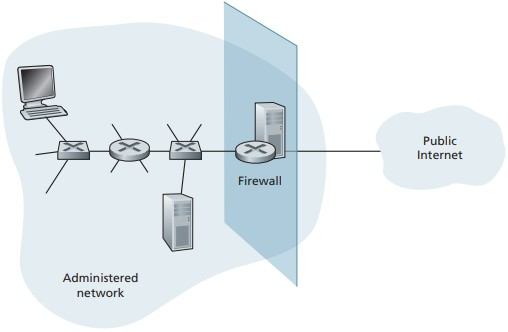
\includegraphics[width=0.95\linewidth]{cap22/packet_filter.png}
\end{minipage}\hfill
\begin{minipage}{0.51\linewidth}
\begin{itemize}
  \item \textbf{Tutto} il traffico in entrata e in uscita dovrebbe passare per il firewall, e solo il traffico \textbf{autorizzato} (secondo la politica di
        sicurezza locale) può passare.
  \item Il firewall fa da \textbf{unico punto di accesso} alla rete pubblica, ma le grandi organizzazioni possono avere più livelli di firewall o
        firewall distribuiti.
  \item Il firewall stesso deve essere \textbf{immune alle intrusioni}: se viene compromesso, dà un falso senso di sicurezza, che è peggio
        di nessuna sicurezza.
  \item Ancora \emph{match più azione}: il match sono indirizzi, porte e flag; l'azione è scartare.
\end{itemize}
\end{minipage}
\caption{Un firewall tra la rete amministrata e la rete pubblica.}
\end{figure}

Vediamo tre approcci: il \textbf{filtraggio tradizionale} dei pacchetti, il \textbf{filtraggio stateful} e l'\textbf{application gateway}.

% ══════════════════════════════════════════════════════════════
\section{Il filtraggio tradizionale dei pacchetti}
% ══════════════════════════════════════════════════════════════

\begin{itemize}
    \item Un \textbf{filtro di pacchetti} è di solito realizzato sul \textbf{gateway}, il router che collega la rete locale all'ISP.
    \item Esamina \textbf{ogni singolo datagramma} e decide se accettarlo o scartarlo in base a regole specificate dall'amministratore. Si possono avere
          regole diverse per i datagrammi in entrata e in uscita, o per le singole interfacce.
\end{itemize}

Le regole si basano tipicamente su:

\begin{itemize}
    \item indirizzo IP sorgente o destinazione;
    \item tipo di protocollo nel campo del datagramma IP (TCP, UDP, ICMP, OSPF);
    \item porta sorgente e destinazione;
    \item bit dei flag TCP (SYN, ACK, \dots) e tipo dei messaggi ICMP;
    \item direzione, e interfaccia.
\end{itemize}

Niente oltre l'header di trasporto: è ciò che lo rende veloce, ed è ciò che lo limita.

\begin{table}[H]
\centering
\begin{tabular}{p{6cm}p{8cm}}
\toprule
\textbf{Politica} & \textbf{Regola} \\
\midrule
Solo il nostro server Web accetta connessioni & scartare i SYN in entrata se non diretti a \texttt{130.207.244.203:80} \\
Le Web radio non devono mangiarsi la banda & scartare l'UDP in entrata, DNS escluso \\
Non rispondiamo ai ping dall'esterno & scartare le echo request ICMP in entrata \\
Non fare da amplificatore per uno smurf & scartare i ping verso un indirizzo di broadcast \\
Nessuno fa traceroute della nostra rete & scartare gli ICMP \emph{TTL expired} in uscita \\
\bottomrule
\end{tabular}
\caption{Dalla politica alle regole.}
\end{table}

\begin{itemize}
    \item Scartare i segmenti in entrata con \textbf{ACK = 0}: nessuno dall'esterno può aprire una connessione, e i client interni
          possono ancora farlo.
    \item Si scartano gli ICMP che si deve, non tutti: la scoperta della MTU del percorso vive di \emph{fragmentation needed}.
\end{itemize}

\warning{I filtri non proteggono dallo spoofing}{
    Politiche basate su indirizzi e porte non proteggono dallo \textbf{spoofing}: un pacchetto con indirizzo sorgente falsificato su quello di un host
    fidato passa il filtro.
}

\subsection{Le access control list}

Nei router le regole del firewall sono realizzate con le \textbf{access control list} (ACL). Consideriamo l'ACL dell'interfaccia che collega il
router all'ISP, per un'organizzazione con indirizzi \texttt{222.22/16} che vuole lasciar passare \textbf{solo il traffico Web}:

\begin{table}[H]
\centering
\small
\begin{tabular}{lllllll}
\toprule
\textbf{Azione} & \textbf{IP sorgente} & \textbf{IP destinazione} & \textbf{Protocollo} & \textbf{Porta sorg.} & \textbf{Porta dest.} & \textbf{Flag} \\
\midrule
allow & 222.22/16 & esterno a 222.22/16 & TCP & $>$ 1023 & 80 & qualsiasi \\
allow & esterno a 222.22/16 & 222.22/16 & TCP & 80 & $>$ 1023 & ACK \\
allow & 222.22/16 & esterno a 222.22/16 & UDP & $>$ 1023 & 53 & --- \\
allow & esterno a 222.22/16 & 222.22/16 & UDP & 53 & $>$ 1023 & --- \\
deny & tutto & tutto & tutto & tutto & tutto & tutto \\
\bottomrule
\end{tabular}
\caption{Una ACL che permette solo il traffico Web (le regole si leggono dall'alto: vale la prima che corrisponde).}
\end{table}

\begin{enumerate}
    \item La prima regola lascia \textbf{uscire} qualsiasi pacchetto TCP con porta di destinazione 80.
    \item La seconda lascia \textbf{entrare} qualsiasi pacchetto TCP con porta sorgente 80 e flag \textbf{ACK = 1} (tutti i messaggi Web di risposta portano
          un ACK, mentre un tentativo di aprire una connessione dall'esterno avrebbe SYN senza ACK).
    \item La terza e la quarta insieme permettono ai pacchetti \textbf{DNS} di uscire ed entrare (senza DNS non si navigherebbe).
    \item L'ultima nega tutto il resto.
\end{enumerate}

C'è una lista per ogni interfaccia del router, letta dall'alto in basso: decide la prima regola che corrisponde, e l'ultima nega tutto
il resto.

\warning{Un'ACL per il Web di ieri}{
    La lista dovrebbe permettere all'organizzazione di navigare. Un browser dietro di essa funziona oggi? Quasi per niente: quasi ogni sito
    sta sulla porta \textbf{443}, e i browser rifiutano l'HTTP in chiaro prima ancora che parta un pacchetto: la lista li blocca tutti. E
    una risposta DNS troppo grande per UDP viene ritentata su TCP porta 53: scartata anche quella, e un nome fallisce senza motivo
    visibile. Un insieme di regole è una fotografia di quali porte portavano che cosa il giorno in cui è stato scritto. Le porte sono
    convenzioni: un'applicazione può usarne qualsiasi, e la cifratura nasconde ciò che portano.
}

\subsection{Il limite: il filtraggio è stateless}

\warning{Pacchetti ACK falsi}{
    Il filtraggio tradizionale è \textbf{senza stato}: esamina ogni pacchetto da solo. Per quanto restrittiva, la tabella precedente lascia entrare
    \textbf{qualsiasi} pacchetto dall'esterno con ACK = 1 e porta sorgente 80, anche se non fa parte di nessuna connessione aperta dall'interno.
    Pacchetti di questo tipo portano payload malformati, alimentano un denial of service e servono a mappare l'interno: chi risponde rivela
    un host. La soluzione ingenua sarebbe bloccare anche i pacchetti TCP ACK, ma impedirebbe agli utenti interni di navigare sul Web. Ciò
    che manca al filtro è la \textbf{memoria}: qualcuno all'interno ha aperto questa connessione?
}

% ══════════════════════════════════════════════════════════════
\section{Il filtraggio stateful}
% ══════════════════════════════════════════════════════════════

\dfn{Filtro stateful}{
    I \textbf{filtri stateful} risolvono il problema tenendo traccia di \textbf{tutte le connessioni TCP in corso} in una \textbf{tabella delle
    connessioni}, per capire se il traffico appartiene a una connessione legittima.
    \begin{itemize}
      \item Il firewall riconosce l'\textbf{inizio} di una nuova connessione (la sequenza SYN, SYNACK, ACK del three-way handshake) e la sua
            \textbf{fine} (il pacchetto FIN).
      \item Può anche assumere (in modo conservativo) che la connessione sia finita quando non vede attività per un certo tempo (per esempio 60 secondi).
    \end{itemize}
}

\begin{figure}[H]
    \centering
    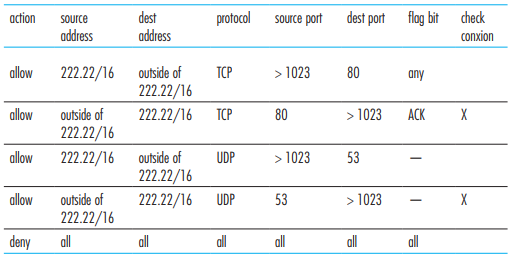
\includegraphics[width=0.65\linewidth]{cap22/stateful_table.png}
    \caption{L'ACL di un filtro stateful: la colonna ``check connection'' indica le regole che richiedono di verificare la tabella delle connessioni. In questo caso sono ammessi solo i pacchetti ACK che appartengono a connessioni già stabilite.}
\end{figure}

Una tabella stateful ha di solito una colonna ``\emph{check connection}'' che indica se un pacchetto deve far parte di una connessione già
stabilita: un pacchetto con ACK = 1 in arrivo dall'esterno passa solo se nella tabella c'è una connessione aperta dall'interno con gli stessi
indirizzi e porte. L'ACK falsificato non ne trova nessuna, la risposta vera sì.

\subsection{La tabella delle connessioni sulla propria macchina}

\begin{lstlisting}[language=bash]
$ sudo conntrack -L -p tcp --dport 443          # una riga, spezzata qui
tcp 6 431996 ESTABLISHED src=192.168.1.23 dst=143.225.161.30 sport=51514 dport=443
    src=143.225.161.30 dst=192.168.1.23 sport=443 dport=51514 [ASSURED] mark=0 use=1
$ sudo nft list chain inet filter input
table inet filter {
    chain input {
        type filter hook input priority filter; policy drop;
        ct state established,related accept      # la colonna check connection
        iif "lo" accept
        tcp dport 22 accept
    }
}
\end{lstlisting}

\begin{itemize}
    \item È la tabella del libro, su una macchina Linux: entrambe le direzioni di ogni connessione, con il suo stato.
    \item Lo stato è l'opinione del filtro, costruita dai segmenti che ha visto: non lo stato TCP di nessuno dei due estremi.
\end{itemize}

% ══════════════════════════════════════════════════════════════
\section{L'application gateway}
% ══════════════════════════════════════════════════════════════

I filtri visti finora controllano soprattutto indirizzi IP e porte. Ma può servire permettere o negare funzionalità in base agli \textbf{utenti} o
all'\textbf{applicazione}, per esempio:

\begin{itemize}
    \item solo i tecnici possono usare certi protocolli (come Telnet verso l'esterno), negati agli utenti normali;
    \item all'interno di un protocollo sono permessi solo certi tipi di messaggi o comandi.
\end{itemize}

Compiti del genere vanno oltre le capacità dei filtri tradizionali e stateful: l'identità degli utenti interni è un dato applicativo, e non compare
negli header IP/TCP/UDP.

\dfn{Application gateway}{
    Un \textbf{application gateway} (o \emph{application-level gateway}, ALG) permette di filtrare i pacchetti in base ai \textbf{dati di livello
    applicativo}. È realizzato di solito come un \textbf{server separato} che lavora insieme al firewall.
}

\begin{figure}[H]
\centering
\begin{minipage}{0.4\linewidth}\centering
  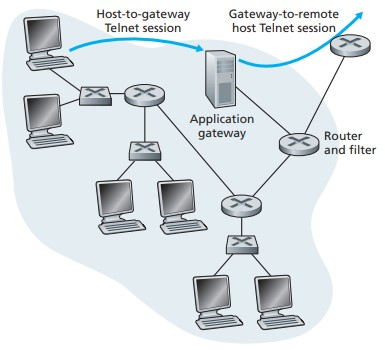
\includegraphics[width=0.95\linewidth]{cap22/app_gateway.png}
\end{minipage}\hfill
\begin{minipage}{0.56\linewidth}
\begin{itemize}
  \item L'idea è \textbf{negare tutte le connessioni} di un certo protocollo (per esempio Telnet) \textbf{tranne} quelle da e verso l'application gateway.
  \item Un utente che vuole usare il protocollo ristretto deve prima \textbf{autenticarsi presso il gateway} (nome utente e password).
  \item Il server controlla se l'utente ha il permesso per quel protocollo.
  \item Se sì, tutte le richieste e le risposte vengono inoltrate attraverso il gateway (che fa da \textbf{proxy}).
\end{itemize}
Le reti interne hanno spesso più application gateway, per protocolli diversi (Telnet, HTTP, FTP, posta).
\end{minipage}
\caption{Un gateway per Telnet: sessione host--gateway e sessione gateway--host remoto, con un router che filtra tutto il resto.}
\end{figure}

\warning{Gli svantaggi}{
    \begin{itemize}
      \item Serve un application gateway \textbf{diverso per ogni applicazione}: Telnet, HTTP e posta hanno ciascuno il suo.
      \item Ogni byte viene inoltrato due volte: una \textbf{penalità di prestazioni} che cresce con il numero di utenti.
      \item Il software sugli host deve sapere che il gateway esiste, e come dirgli dove andare.
    \end{itemize}
}

Ne avete già incontrati due: il server di posta di un'organizzazione e la sua cache Web sono application gateway. Il gateway Telnet di
oggi è un \textbf{bastion host} SSH: l'unica macchina raggiungibile dall'esterno, dove gli utenti si autenticano prima di andare oltre
(\emph{autorizzazione}, dopo l'autenticazione).

% ══════════════════════════════════════════════════════════════
\section{Gli Intrusion Detection System}
% ══════════════════════════════════════════════════════════════

Per rilevare certi tipi di attacco serve un'\textbf{ispezione profonda dei pacchetti} (\emph{deep packet inspection}): controllare, anche nel
contenuto, schemi di attacco noti o traffico sospetto.

\dfn{IDS e IPS}{
    Un \textbf{Intrusion Detection System} (IDS) è un insieme di dispositivi specializzati che \textbf{monitorano la rete} cercando pacchetti sospetti.
    \begin{itemize}
      \item Il suo compito principale è \textbf{riconoscere} i pacchetti potenzialmente malevoli e \textbf{allertare} l'amministratore di rete (che poi
            deciderà cosa fare).
      \item Se può anche \textbf{bloccare} (filtrare) i pacchetti sospetti, si parla di \textbf{Intrusion Prevention System} (IPS).
    \end{itemize}
}

Le organizzazioni usano gli IDS per rilevare un'ampia gamma di attacchi (o di potenziali attacchi):

\begin{itemize}
    \item scansioni della rete o delle porte (per esempio con nmap);
    \item flooding DoS;
    \item worm e virus, e sfruttamento di vulnerabilità note.
\end{itemize}

\begin{itemize}
    \item Un IPS deve stare \textbf{sul percorso} e decidere subito; un IDS può osservare una copia del traffico da parte.
    \item Perché non bloccare sempre? Un falso allarme che uccide una connessione legittima costa più di un avviso che qualcuno legge.
    \item \textbf{Di rete o di host}: un NIDS sorveglia molte macchine; un HIDS ne sorveglia una, dopo decifratura e riassemblaggio.
\end{itemize}

\begin{figure}[H]
    \centering
    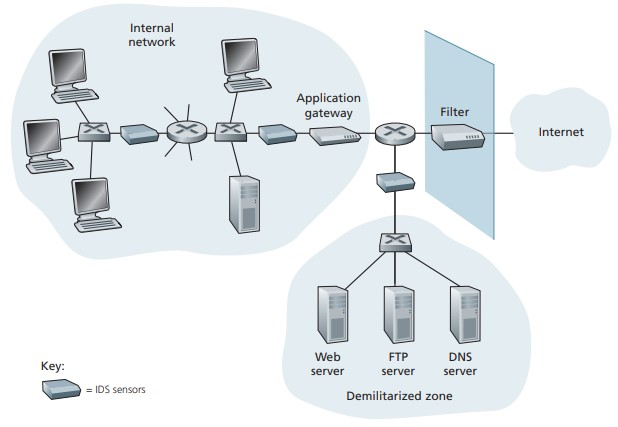
\includegraphics[width=0.65\linewidth]{cap22/ids.png}
    \caption{Una rete con filtro, application gateway, sensori IDS e zona demilitarizzata (da Kurose).}
\end{figure}

Il sistema è spesso composto da:

\begin{itemize}
    \item uno o più \textbf{sensori IDS};
    \item un unico \textbf{processore IDS centrale}, che raccoglie e integra le informazioni e invia gli allarmi.
\end{itemize}

Gli IDS possono essere:

\begin{itemize}
    \item \textbf{basati su firme} (\emph{signature-based}): mantengono un ampio database di \textbf{firme di attacco}, cioè insiemi di regole legate a
          un'attività di intrusione (è il tipo più comune). Non riconoscono attacchi nuovi;
    \item \textbf{basati su anomalie} (\emph{anomaly-based}): costruiscono un \textbf{profilo del traffico} normale e segnalano i flussi statisticamente
          insoliti. Possono scoprire attacchi nuovi, ma spiegano poco, ed è difficile distinguere il traffico anomalo da quello semplicemente raro.
\end{itemize}

\subsection{Una firma, letta campo per campo}

\begin{lstlisting}[language=bash]
alert icmp $EXTERNAL_NET any -> $HOME_NET any
      (msg:"ICMP PING NMAP"; dsize: 0; itype: 8;)
\end{lstlisting}

\begin{itemize}
    \item \texttt{alert icmp}: genera un allarme su un pacchetto ICMP, dall'esterno dell'organizzazione verso la sua rete.
    \item \texttt{itype: 8} è una echo request; \texttt{dsize: 0} un payload vuoto. Il vostro ping porta 56 byte.
    \item nmap trova gli host di altre reti con echo request vuote; sulla propria subnet chiede invece ad ARP.
    \item La comunità di Snort pubblica una firma poche ore dopo un nuovo attacco, e i sensori la scaricano ovunque.
\end{itemize}

\warning{Un allarme che ha ragione il 99\% delle volte}{
    L'IDS individua il 99\% degli attacchi e segnala per errore l'1\% degli eventi normali. Un evento su 100\,000 è un attacco. Suona un
    allarme: quanto è probabile che sia un attacco? Circa \textbf{uno su mille}:
    $$\frac{0{,}00001 \cdot 0{,}99}{0{,}00001 \cdot 0{,}99 + 0{,}99999 \cdot 0{,}01} \approx 0{,}001.$$
    Gli eventi normali sono così tanti che il loro 1\% di falsi allarmi seppellisce quelli veri: è la \textbf{fallacia del tasso di base}
    (\emph{base-rate fallacy}). A decidere è il tasso di \textbf{falsi positivi}, non quello di rilevazione; e un amministratore che vede
    mille falsi allarmi per ognuno vero smette di leggerli.
}

\subsection{Ispezionare ciò che è cifrato}

Quasi tutto il traffico oggi è TLS. Che cosa possono ancora leggere un firewall o un IDS? Indirizzi, porte, il nome del server nel Client
Hello, dimensioni e tempi. Il payload, dove le firme trovano corrispondenze, è sparito: una protezione acceca l'altra. Le organizzazioni che
devono ispezionare installano un proprio certificato radice su ogni macchina, e una scatola che termina TLS: un \textbf{man in the middle
per regolamento}, con un certificato valido per qualsiasi sito, emesso da una radice di cui alle macchine è stato detto di fidarsi.

% ══════════════════════════════════════════════════════════════
\section{La zona demilitarizzata (DMZ)}
% ══════════════════════════════════════════════════════════════

Nelle reti grandi capita spesso di dover avere \textbf{due livelli di sicurezza} per dispositivi diversi: i server che devono comunicare con il mondo
esterno, per esempio, hanno bisogno di un filtraggio più blando.

\dfn{Zona demilitarizzata (DMZ)}{
    Una \textbf{zona demilitarizzata} (DMZ) è una regione a \textbf{bassa sicurezza}, con restrizioni limitate, in cui ospitare i server che devono
    essere raggiungibili dall'esterno (Web, FTP, DNS). Un approccio tipico è mettere la DMZ \textbf{tra due firewall}: uno esterno, meno restrittivo, e
    uno interno, più restrittivo.
}

\begin{figure}[H]
\centering
\begin{tikzpicture}[every node/.style={font=\footnotesize\sffamily}]
  \node[netcloud, minimum width=2.4cm] (i) at (0,0) {Internet};
  \node[draw, fill=netred!30, minimum width=0.5cm, minimum height=1.8cm] (f1) at (2.6,0) {};
  \node[below=2pt of f1, align=center] {firewall\\esterno};
  \node[draw=netorange, thick, dashed, rounded corners, fill=netorange!8, minimum width=3.4cm, minimum height=2.4cm] (dmz) at (5.6,0) {};
  \node[anchor=north, text=netorange, font=\footnotesize\bfseries\sffamily] at (dmz.north) {DMZ};
  \node at (4.8,-0.3) {\icon[0.45cm]{server}}; \node at (5.6,-0.3) {\icon[0.45cm]{server}}; \node at (6.4,-0.3) {\icon[0.45cm]{server}};
  \node[font=\scriptsize\sffamily] at (5.6,-0.95) {Web \quad FTP \quad DNS};
  \node[draw, fill=netred!60, minimum width=0.5cm, minimum height=1.8cm] (f2) at (8.6,0) {};
  \node[below=2pt of f2, align=center] {firewall interno\\+ app. gateway};
  \node[draw=netgreen!60!black, thick, rounded corners, fill=netgreen!8, minimum width=3.2cm, minimum height=2.4cm] (lan) at (11.6,0) {};
  \node[anchor=north, text=netgreen!50!black, font=\footnotesize\bfseries\sffamily] at (lan.north) {rete interna};
  \node at (11,-0.3) {\icon[0.6cm]{pc}}; \node at (12.1,-0.3) {\icon[0.7cm]{laptop}};
  \draw[wired] (i) -- (f1); \draw[wired] (f1) -- (dmz); \draw[wired] (dmz) -- (f2); \draw[wired] (f2) -- (lan);
  \node[text width=4cm, align=center, text=netred] at (5.6,-1.8) {filtraggio blando, sensori IDS};
  \node[text width=4cm, align=center, text=netgreen!50!black] at (11.6,-1.8) {alta sicurezza, sensori IDS};
\end{tikzpicture}
\caption{La DMZ tra due firewall.}
\end{figure}

\begin{itemize}
    \item La regione ad \textbf{alta sicurezza} è protetta da un filtro di pacchetti e da un application gateway, ed è monitorata da sensori IDS.
    \item La regione a \textbf{bassa sicurezza} (la DMZ) è protetta solo dal filtro ed è monitorata dai sensori: Web, posta, DNS autoritativo.
    \item Un server violato nella DMZ non è ancora dentro: \textbf{difesa in profondità}, fino a ogni singolo host.
    \item Nessun perimetro ferma chi è già dentro.
\end{itemize}

\info{TLS nasconde che cosa si dice, non a chi}{
    Crittografia e firewall proteggono i contenuti, ma chi osserva la rete vede comunque \textbf{chi} parla con \textbf{chi}. Nascondere anche
    questo è l'argomento del prossimo capitolo.
}

\begin{esercizio}{Firme, record e allarmi}
\begin{enumerate}[label=(\alph*)]
    \item Alice riceve da Bob $m$ e $K_B^-(H(m))$. Quali passi esegue, e che cosa sa se il controllo riesce? Che cosa \textbf{non} sa?
    \item In una sessione TLS Trudy elimina il record numero 3 inviato da Bob. Che cosa succede quando arriva il record 4?
    \item Un IDS rileva il 99,9\% degli attacchi con lo 0,1\% di falsi positivi, e un evento su 10\,000 è un attacco. Qual è la
          probabilità che un allarme sia vero?
    \item Nell'ACL ``solo Web'', quale regola lascia entrare un segmento con porta sorgente 80, ACK = 1 e nessuna connessione dietro? Come lo
          ferma un filtro stateful?
\end{enumerate}

\svolgimento
\begin{enumerate}[label=(\alph*)]
    \item Calcola $H(m)$, applica la chiave pubblica di Bob alla firma, $K_B^+(K_B^-(H(m)))$, e confronta. Se sono uguali, $m$ è integro ed è
          stato firmato da chi possiede la chiave privata corrispondente a quella pubblica usata. Non sa, senza un certificato, che quella
          chiave pubblica sia davvero di Bob (la pizza), né che il messaggio sia fresco.
    \item Il ricevente si aspetta il contatore 3, ma l'HMAC del record arrivato è stato calcolato con il contatore 4: il controllo fallisce e
          la connessione viene chiusa con un errore.
    \item $\dfrac{0{,}0001 \cdot 0{,}999}{0{,}0001 \cdot 0{,}999 + 0{,}9999 \cdot 0{,}001} \approx \dfrac{0{,}0000999}{0{,}0010998}
          \approx 0{,}09$: circa 9 allarmi su 100.
    \item La seconda (TCP da porta 80 verso porte $>$ 1023 con ACK). Un filtro stateful la marca ``check connection'': il segmento passa solo
          se nella tabella c'è una connessione aperta dall'interno con gli stessi indirizzi e porte, e qui non c'è.
\end{enumerate}
\end{esercizio}

\Needspace{20\baselineskip}
% ══════════════════════════════════════════════════════════════
\section{Riepilogo}
% ══════════════════════════════════════════════════════════════

\riepilogo{
\begin{itemize}
    \item Una \textbf{firma} è un hash sotto una chiave privata: chiunque la verifica, uno solo poteva produrla. Un \textbf{certificato} è la
          firma di una CA, in una catena fino a una radice.
    \item \textbf{Autenticazione}: servono un segreto e la freschezza. L'IP si falsifica, la password si intercetta, la password cifrata si
          ripete (\textbf{playback}); il \textbf{nonce} mostra che l'altra parte c'è adesso.
    \item \textbf{TLS}: un certificato per fidarsi del server (con il nome giusto), un handshake per le chiavi, record con HMAC e contatore,
          un record di chiusura. La versione 1.3 firma un Diffie-Hellman: forward secrecy.
    \item \textbf{Firewall}: filtrano gli header, da soli (ACL) o con una tabella delle connessioni (stateful); gli \textbf{application
          gateway} filtrano utenti e contenuti.
    \item \textbf{IDS/IPS}: leggono i payload e danno l'allarme; il loro nemico è il falso positivo, e la cifratura li acceca. La
          \textbf{DMZ} ospita i server pubblici.
    \item TLS nasconde che cosa si dice, non a chi lo si dice.
\end{itemize}
}
